%-----------------------------------LICENSE------------------------------------%
%   This file is part of Mathematics-and-Physics.                              %
%                                                                              %
%   Mathematics-and-Physics is free software: you can redistribute it and/or   %
%   modify it under the terms of the GNU General Public License as             %
%   published by the Free Software Foundation, either version 3 of the         %
%   License, or (at your option) any later version.                            %
%                                                                              %
%   Mathematics-and-Physics is distributed in the hope that it will be useful, %
%   but WITHOUT ANY WARRANTY; without even the implied warranty of             %
%   MERCHANTABILITY or FITNESS FOR A PARTICULAR PURPOSE.  See the              %
%   GNU General Public License for more details.                               %
%                                                                              %
%   You should have received a copy of the GNU General Public License along    %
%   with Mathematics-and-Physics.  If not, see <https://www.gnu.org/licenses/>.%
%------------------------------------------------------------------------------%
%   Author:     Ryan Maguire                                                   %
%   Date:       February 17, 2022                                              %
%------------------------------------------------------------------------------%
\documentclass{beamer}
\usepackage{amsmath}

\title{Conjectures on Khovanov and Knot Floer Homology and an Algorithm
       for the Jones Polynomial}
\author{Ryan Maguire}
\date{February 17, 2022}
\usenavigationsymbolstemplate{}
\setbeamertemplate{footline}[frame number]
\begin{document}
    \maketitle
    \begin{frame}{\textbf{\color{red}{Corrections}}}
        A bug was discovered in the Knot Floer Homology (KFH) code that led to
        false negatives. The conjecture as presented in this talk for
        KFH and Legendrian simple knots is false and counterexamples have been
        found. For Khovanov homology the conjecture still stands as of this
        correction (written 2023/02/27).
        \par\hfill\par
        The wording of the theorem about Gauss codes has been corrected, and
        references given.
        \par\hfill\par
        The remainder of these slides are unchanged from the original talk.
    \end{frame}
    \begin{frame}{Outline}
        \begin{itemize}
            \item Gauss Code
            \item The Kauffman Bracket and Jones Polynomial
            \item Khovanov Homology
            \item An Algorithm for the Jones Polynomial
            \item Conjectures on Khovanov and Knot Floer Homology
        \end{itemize}
    \end{frame}
    \begin{frame}{Gauss Code}
        Take a knot, orient it, and label the crossings from 0 to $N-1$.
        Starting at the 0 crossing, travel along the knot and when you come
        to a crossing, record the crossing number and whether you're on the
        \textit{over} strand or the \textit{under} strand. The string of length
        $2N$ you've obtained is the \textit{Gauss code} of the knot.
        \begin{figure}
            \centering
            \resizebox{0.3\textwidth}{!}{%
                \includegraphics{%
                    ../images/trefoil_knot_oriented_with_gauss_code.pdf%
                }
            }
            \caption{Gauss Code for the Right-Handed Trefoil}
            \label{fig:right_handed_trefoil_gauss_code}
        \end{figure}
    \end{frame}
    \begin{frame}{Gauss Code}
        Problem: Different knots can have the same Gauss code.%
        \footnote{%
            It bothers me that there's only \textit{one} trefoil knot in every
            knot table.
        }
        Take the left-handed trefoil, similar orientation and labelling scheme
        as before, but different starting point. The resulting code is the same
        as before. The left and right handed Trefoils are different
        (Their Jones polynomials are different).%
        \footnote{
            Did it really take until the 1980's to know these are different?
        }
        \begin{figure}
            \centering
            \resizebox{0.3\textwidth}{!}{%
                \includegraphics{%
                    ../images/trefoil_knot_mirror_oriented_with_gauss_code.pdf%
                }
            }
            \caption{Gauss Code for the Left-Handed Trefoil}
            \label{fig:left_handed_trefoil_gauss_code}
        \end{figure}
    \end{frame}
    \begin{frame}{Gauss Code}
        \begin{theorem}
            If two classical prime knots have the same Gauss code, either they
            are isomorphic, or they are mirrors of each other.
        \end{theorem}
        By \textit{classical} it is meant that the knots are not virtual
        (discussed in a few slides). Dowker and Thistlethwaite proved that DT
        code uniquely specifies a prime knot up to reflection
        \cite{DOWKER198319}, and DT codes
        contain the same information as Gauss codes. Indeed, there are
        algorithms to go from one to the other \cite{KatlasDTCodes}.
        \par\hfill\par
        We have an example of two distinct knots having the same Gauss code,
        the left and right handed trefoils. How can we describe knots while
        distinguishing mirrors?
    \end{frame}
    \begin{frame}{Gauss Code}
        Solution: Sign the crossings. At every crossing, rotate your head until
        the crossing looks like one of the ones below. Call the one on the left
        a \textit{negative crossing} and the one on the right \textit{positive}.
        \begin{figure}
            \centering
            \includegraphics{../images/crossing_signs.pdf}
            \caption{Crossing Signs}
            \label{fig:crossing_signs}
        \end{figure}
    \end{frame}
    \begin{frame}{Gauss Code}
        By also recording the sign, we get \textit{extended Gauss code}.
        \begin{theorem}
            If two classical prime knots have the same extended Gauss code,
            they are isomorphic.
        \end{theorem}
        Since unsigned codes distinguish knots up to mirror equivalence, and
        since signing the code detects mirrors, the result is almost immediate.
    \end{frame}
    \begin{frame}{Gauss Code}
        Below is the extended Gauss code for the right-handed trefoil.
        \begin{figure}
            \centering
            \includegraphics{%
                ../images/trefoil_knot_oriented_with_extended_gauss_code.pdf%
            }
            \caption{Extended Gauss Code for the Right-Handed Trefoil}
            \label{fig:right_hand_trefoil_extended_gauss}
        \end{figure}
    \end{frame}
    \begin{frame}{Gauss Code}
        The rules:
        \begin{enumerate}
            \item Gauss code is a finite sequence of length $2N$ of ordered
                  triples.
            \item The ordered triples are of the form $(s,n,t)$ with
                  $s\in\{-1,+1\}$, $t\in\{O,U\}$, and $0\leq{n}\leq{N-1}$.
                  ($s$ for \textit{sign}, $t$ for \textit{type}).
            \item Every integer $0\leq{n}\leq{N-1}$ occurs exactly twice in the
                  code, once with $O$ and once with $U$. The sign does not
                  change.
        \end{enumerate}
    \end{frame}
    \begin{frame}{Gauss Code}
        The three Reidemeister moves translate to fairly simple operations on
        Gauss code.\footnote{HW what are they?}
        We will be discussing an algorithm for the Jones polynomial that is
        exponential in crossings and it would be nice if there were a simpler
        knot than either of the trefoils. And there is!
        \begin{equation}
            O0\;O1\;U0\;U1
        \end{equation}
        You'll find no Reidemeister moves can reduce this to the unknot.
    \end{frame}
    \begin{frame}{Gauss Code}
        If you try to draw the knot from this code, you'll get the following.
        There's this \textit{fake} crossing.
        \begin{figure}
            \centering
            \includegraphics{../images/chain_link_fence_knot_virtual.pdf}
            \caption{The Chain Link Fence Knot}
            \label{fig:chain_link_fence_knot}
        \end{figure}
    \end{frame}
    \begin{frame}{Gauss Code}
        The graph theorist in you knows that we really want to draw this on a
        torus.%
        \footnote{Ever try and draw $K_{5}$ without crossings?}
        \begin{figure}
            \centering
            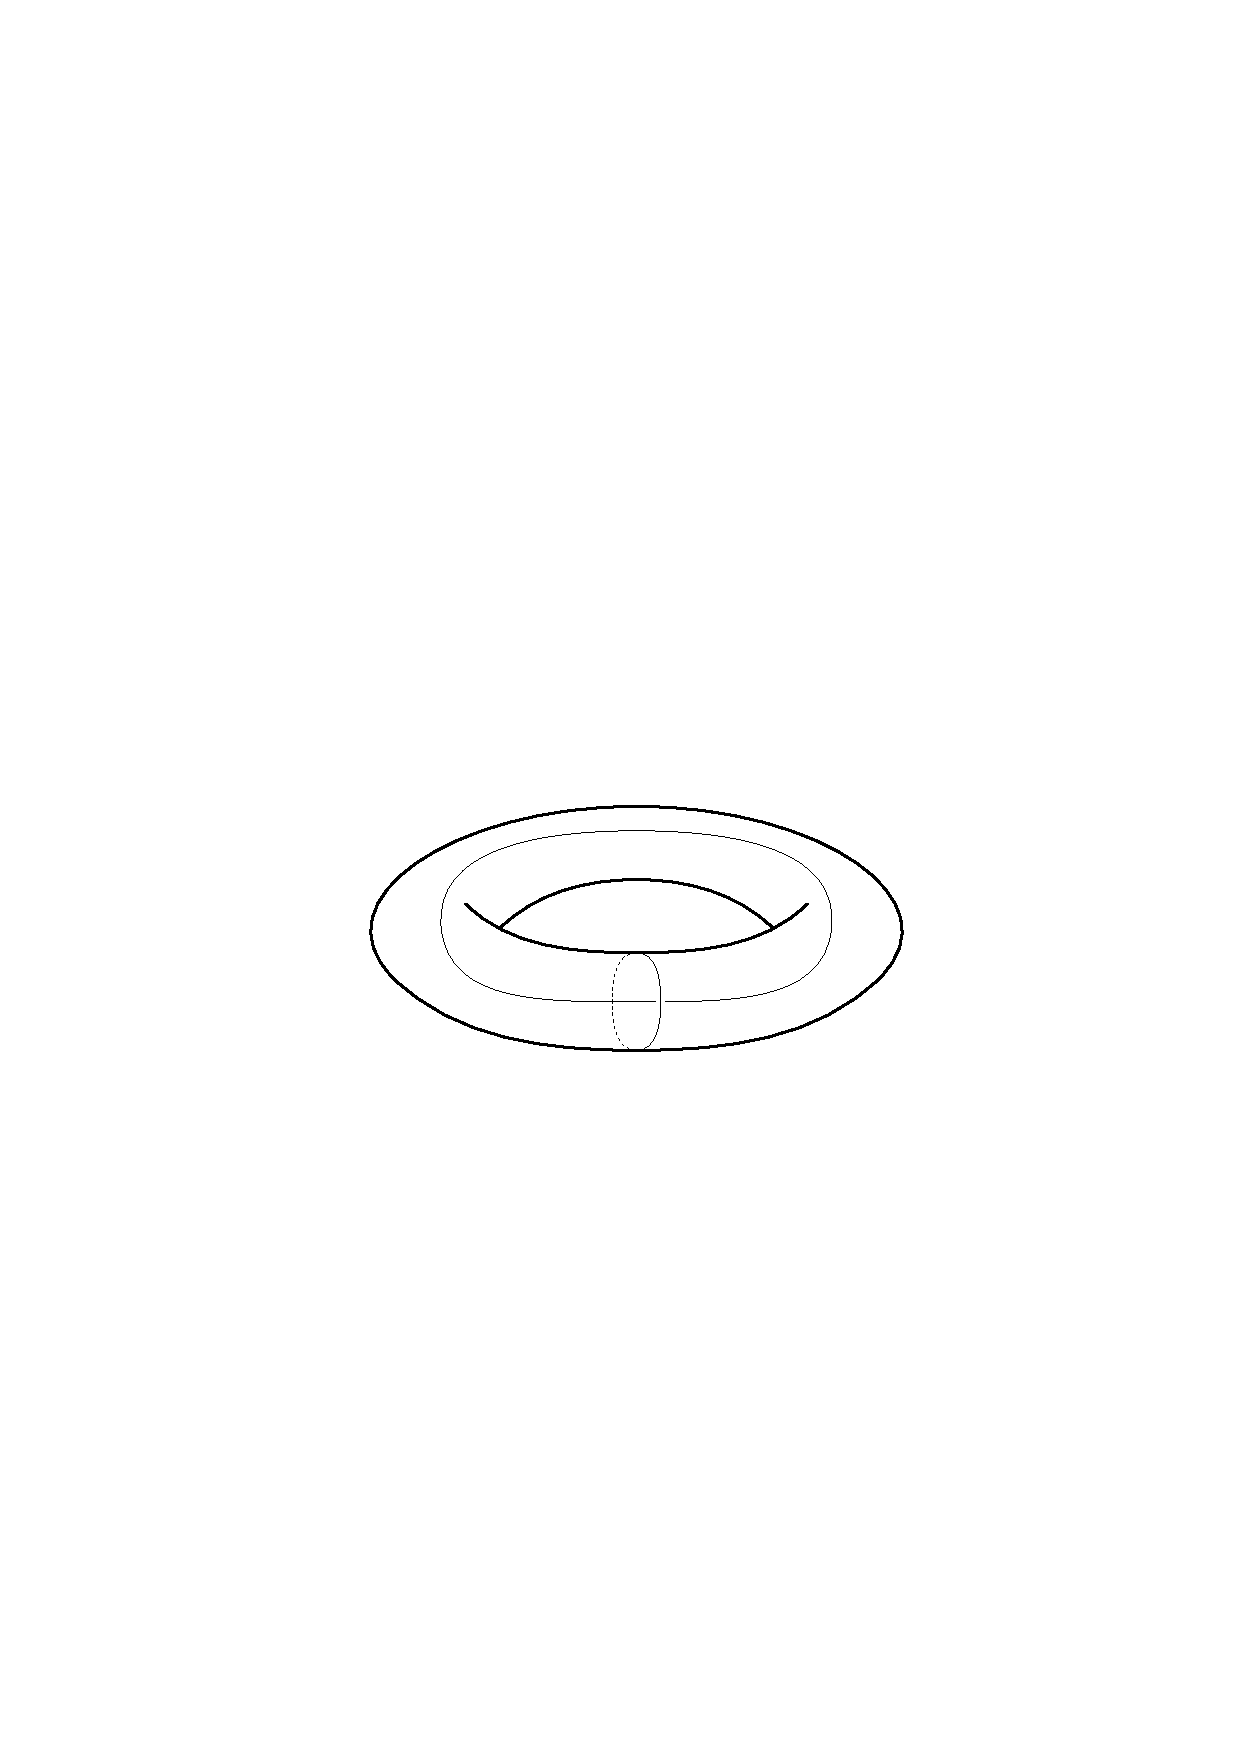
\includegraphics{../images/chain_link_fence_knot_on_torus.pdf}
            \caption{The Chain Link Fence Knot on a Torus}
            \label{fig:chain_link_fence_knot_on_torus}
        \end{figure}
    \end{frame}
    \begin{frame}{Gauss Code}
        But what shall we name it (don't read the figures label)?
        Let's draw it on a flat torus.
        \begin{figure}
            \centering
            \includegraphics{../images/chain_link_fence_knot_on_flat_torus.pdf}
            \caption{The Chain Link Fence Knot on a Flat Torus}
            \label{fig:chain_link_fence_knot_on_flat_torus}
        \end{figure}
    \end{frame}
    \begin{frame}{Gauss Code}
        And then let's lift that drawing to the universal cover.
        \begin{figure}
            \centering
            \resizebox{0.6\textwidth}{!}{%
                \includegraphics{%
                    ../images/chain_link_fence_knot_on_flat_torus_universal_cover.pdf%
                }%
            }
            \caption{Lift of the Chain Link Fence Knot to $\mathbb{R}^{2}$}
            \label{fig:chain_link_fence_knot_on_flat_torus_universal_cover}
        \end{figure}
    \end{frame}
    \begin{frame}{Gauss Code}
        Looks like a chain-link fence. Let's call it that. This is the simplest
        non-trivial \textit{virtual knot}. A classical knot can be thought of
        as a smooth embedding of $\mathbb{S}^{1}$ into
        $\mathbb{S}^{2}\times\mathbb{R}$. Virtual knots are smooth embeddings
        of $\mathbb{S}^{1}$ into $M\times\mathbb{R}$ where $M$ is a compact
        surface. The \textit{virtual genus} of a virtual knot is the smallest
        possible genus of $M$. Classical knots have virtual genus 0. The
        chain-link fence knot has virtual genus 1.
    \end{frame}
    \begin{frame}{Gauss Code}
        We can detect the virtual genus from extended Gauss code. Take the
        right-handed trefoil and thicken it. Start anywhere you'd like, but
        place your finger on the \textit{left} strand and start walking forward.
        When you encounter a crossing, go left! Eventually you'll end up back
        where you started. Keep doing this until you've traversed all of the
        strands, keeping track of the total number of cycles.
        \begin{figure}
            \centering
            \includegraphics{../images/trefoil_knot_framed_001.pdf}
            \caption{Framed Left-Handed Trefoil}
            \label{fig:trefoil_knot_framed_001}
        \end{figure}
    \end{frame}
    \begin{frame}{Gauss Code}
        To conclude, use the following:
        \begin{equation}
            V-E+F=2-2g
        \end{equation}
        You've just computed $F$! $V$ is the number of crossings, and
        $E$ is always $2V$ (the knot graph is a four-valent multigraph. By the
        hand-shaking theorem, $E=4V/2=2V$). So:
        \begin{equation}
            g=\frac{V-F+2}{2}
        \end{equation}
        We don't care about the virtual genus right now. But we do care about
        the idea. We will modify it later to get the Jones polynomial.
    \end{frame}
    \begin{frame}{The Kauffman Bracket and Jones Polynomial}
        The Kauffman Bracket is defined recursively in terms of smoothings of a
        crossing. Given a crossing, there are two ways to make it
        \textit{go away}. We will label these the 0 and 1 smoothings, see below.
        \begin{figure}
            \centering
            \includegraphics{../images/resolving_crossings.pdf}
            \caption{Resolving a Crossing}
            \label{fig:resolving_crossing}
        \end{figure}
    \end{frame}
    \begin{frame}{The Kauffman Bracket and Jones Polynomial}
        Given a knot with $N$ crossings, with crossings labeled 0 to $N-1$,
        and any integer $0\leq{n}\leq{2}^{N}-1$, there is a unique resolution of
        all crossings corresponding to $n$. Write $n$ in binary. The value of
        the $k^{th}$ bit tells us how we are supposed to smooth the $k^{th}$
        crossing.
        \begin{figure}
            \centering
            \resizebox{0.8\textwidth}{!}{%
                \includegraphics{../images/trefoil_knot_cube_of_resolutions.pdf}
            }
            \caption{Cube of Resolutions for the Left-Handed Trefoil}
            \label{fig:trefoil_knot_cube_of_resolutions}
        \end{figure}
    \end{frame}
    \begin{frame}{The Kauffman Bracket and the Jones Polynomial}
        The following took too long to make.
        \begin{figure}
            \centering
            \resizebox{0.5\textwidth}{!}{%
                \includegraphics{%
                    ../images/figure_eight_knot_cube_of_resolutions.pdf%
                }%
            }
            \caption{Cube of Resolutions for the Figure-Eight}
            \label{fig:figure_eight_knot_cube_of_resolutions}
        \end{figure}
    \end{frame}
    \begin{frame}
        The Kauffman bracket is defined recursively as follows:
        \begin{align}
            \langle\emptyset\rangle&=1\\
            \langle{L\sqcup\mathbb{S}^{1}}\rangle&=(q+q^{-1})\langle{L}\rangle\\
            \langle{L}\rangle&=
                \langle{L_{n,0}}\rangle-q\langle{L_{n,1}}\rangle
        \end{align}
        where $L_{n,0}$ and $L_{n,1}$ are the links obtained from the
        0 and 1 smoothings of $L$ at the $n^{th}$ crossing, respectively. The
        notation $L\sqcup\mathbb{S}^{1}$ means the disjoint union of
        $L$ with an unknot. Hence the Kaufmann bracket of the
        unknot is $q+q^{-1}$.
        \begin{theorem}
            The Kauffman bracket is invariant under Reidemeister II and III
            moves.
        \end{theorem}
        It is not invariant under Reidemeister I, so we have a
        \textit{framed knot} invariant.
    \end{frame}
    \begin{frame}{The Kauffman Bracket and the Jones Polynomial}
        If you have something that is invariant under Reidemeister II and III,
        you should try to introduce the \textit{writhe}%
        \footnote{Sum of the signs of the crossings}
        into the problem since only Reidemeister I changes the writhe of a
        diagram. The Jones polynomial does exactly this:
        \begin{equation}
            J(L)=(-1)^{N_{-}}q^{N_{-}-2N_{+}}\langle{L}\rangle
        \end{equation}
        $N_{\pm}$ being the number of positive and negative crossings,
        respectively.
        \begin{theorem}
            The Jones polynomial is a knot invariant.
        \end{theorem}
    \end{frame}
    \begin{frame}{Khovanov Homology}
        You can get a homology theory out of this. Khovanov homology is the
        ``categorification" of the Jones polynomial, the graded Euler
        characteristic of which gives you the Jones polynomial. I won't be
        discussing heavy details about Khovanov homology, only some of the
        technical difficulties involved in its computation.
        The recursive definition of the chain complex is as follows:
        \begin{align}
            [[\emptyset]]&=0\rightarrow\mathbb{Z}\rightarrow{0}\\
            [[L\sqcup\mathbb{S}^{1}]]&=V\otimes[[L]]\\
            [[L]]&=\mathcal{F}\big(
                0\rightarrow[[L_{n,0}]]\rightarrow[[L_{n,1}]]\{1\}\rightarrow{0}
            \big)
        \end{align}
        $V$ is a graded vector space, $\{\ell\}$ is the
        \textit{degree shift} operation, and $\mathcal{F}$ is the flatten
        operation of graded vector spaces. Like the Kauffman bracket, we need
        the writhe to a get a true knot invariant. The chain complex is
        $C(L)=[[L]][N_{-}]\{N_{-}-2N_{+}\}$, $[\ell]$ is the height shift
        operation on chain complexes. Khovanov homology is the resulting
        homology from this (chain maps are not defined in this talk).
    \end{frame}
    \begin{frame}{Khovanov Homology}
        The na\"{i}ve recursive algorithm for Khovanov homology is exponential
        in both time and space. Most algorithm talks only care about time,
        since in the modern era it seems we have infinite space. The following
        is an excerpt from an email I recently sent:
        \begin{flushright}
            \textit{
                I ran time\footnote{Unix time and memory command}
                to see how much memory the algorithm takes.
                For n=10 and n=12, I get 0.65 GB and 9.33 GB, respectively.
                The algorithm is EXP in space, so I did a best fitting
                exponential. For n=14 (which is what is needed), the output is
                132.5 GB. Yikes.
            }
        \end{flushright}
    \end{frame}
    \begin{frame}{Khovanov Homology}
        No working totally free-and-open-source implementation of a decent
        Khovanov homology algorithm is known to me. There are three existing
        versions, all open source, but each has a problem.
        \begin{itemize}
            \item One is written in Mathematica, which is not an open language.%
                  \footnote{Current pricing options are \$19/month
                            or \$183/year. Ouch.}
            \item Another is written in an old version of Java which wouldn't
                  compile under the latest version of the language.%
                  \footnote{Edit: Nikolay Pultsin recently fixed this and it compiles with OpenJDK-17.}
            \item The sage implementation requires a super computer to actually
                  use (see previous email).
        \end{itemize}
        All efforts are greatly appreciated, but there needs to be a
        \textit{usable} implementation available to the general public without
        costing an arm and a leg.
    \end{frame}
    \begin{frame}{Khovanov Homology}
        Why might we care?
        \begin{itemize}
            \item Khovanov homology is an unknot detector!
                  An efficient algorithm gives a decent means of solving
                  the unknotting problem.
            \item It is a very strong invariant. When trying to tabulate a list
                  of all knots up to $N$ crossings, Khovanov homology can be
                  used to help remove duplicates.
            \item Testing conjectures!
        \end{itemize}
    \end{frame}
    \begin{frame}{An Algorithm for the Jones Polynomial}
        We'll first start with smaller means. We'll tackle the Jones
        polynomial. We'll do this by computing the Kauffman bracket. Using the
        recursive definition we can inductively prove the following formula:
        \begin{equation}
            \label{eqn:kauffman_bracket}%
            \langle{L}\rangle=\sum_{n=0}^{2^{N}-1}
                (-q)^{w(n)}(q+q^{-1})^{c(n)}
        \end{equation}
        Here, $w(n)$ is the \textit{Hamming weight} of $n$, the number of 1's
        that occur in the binary representation of $n$. $c(n)$ is the
        \textit{circle counting function}, the number of disjoint circles that
        result from the complete resolution of $L$ corresponding to $n$.
        To compute $\langle{L}\rangle$ we need only compute $c(n)$.
    \end{frame}
    \begin{frame}{An Algorithm for the Jones Polynomial}
        First, thicken the knot. All of the crossings then become
        ``four-way intersections."
        \begin{figure}
            \centering
            \includegraphics{../images/trefoil_knot_framed_001.pdf}
            \caption{Framed Left-Handed Trefoil}
            \label{fig:trefoil_knot_framed_001}
        \end{figure}
    \end{frame}
    \begin{frame}{An Algorithm for the Jones Polynomial}
        The aforementioned four-way intersections.
        \begin{figure}
            \centering
            \includegraphics{../images/thickened_crossings.pdf}
            \caption{Signed Crossings in a Framed Knot}
            \label{fig:thickened_crossings}
        \end{figure}
    \end{frame}
    \begin{frame}{An Algorithm for the Jones Polynomial}
        A smoothing amounts to a roadblock.
        \begin{figure}
            \centering
            \includegraphics{../images/thickened_negative_crossing_smoothings.pdf}
            \caption{Smoothing a Negative Crossing in a Framed Knot}
            \label{fig:thickened_negative_crossing_smoothings}
        \end{figure}
        \begin{figure}
            \centering
            \includegraphics{../images/thickened_positive_crossing_smoothings.pdf}
            \caption{Smoothing a Positive Crossing in a Framed Knot}
            \label{fig:thickened_positive_crossing_smoothings}
        \end{figure}
    \end{frame}
    \begin{frame}{An Algorithm for the Jones Polynomial}
        Life will be easier if we label the four-way intersection. Given a
        positive or negative crossing, we will label the four roads as follows:
        \begin{figure}
            \centering
            \includegraphics{../images/thickened_crossing_labeled.pdf}
            \caption{Thickened Crossings with Labels}
            \label{fig:thickened_crossings_labeled}
        \end{figure}
        \begin{figure}
            \centering
            \includegraphics{../images/thickened_crossings_resolved_labeled.pdf}
            \caption{Thickened Resolved Crossings with Labels}
            \label{fig:thickened_crossings_resolved_labeled}
        \end{figure}
    \end{frame}
    \begin{frame}{An Algorithm for the Jones Polynomial}
        Create a table with $4N$ entries, all of which are set to 0.
        Start at the 0 crossing in the Gauss code. Pictorially, you are walking
        towards the crossing from road 0. You now need to know which road to
        leave from. Let's suppose the sign of the crossing is negative, and
        you are supposed to do the zero resolution for this crossing. The
        previous figure shows that we must travel down road 1. But hold on,
        the arrows are pointing the wrong way! So we must walk backwards.
        \par\hfill\par
        What does this mean? Find the next entry in the Gauss code for the 0
        crossing (If the first entry is $O0-$, find $U0-$, and vice-versa).
        Since we are walking backwards, from there go to the \textit{previous}
        entry in the Gauss code (that's what walking backwards means). We have
        traversed roads 0 and 1 for the 0 crossing, so change entries 0 and 1 of
        our table to 1.
    \end{frame}
    \begin{frame}{An Algorithm for the Jones Polynomial}
        We continue this idea for all other crossings. We just need to know
        which road to leave from, given the crossing sign, type, and resolution,
        and which road we are entering from for the next crossing. This can be
        obtained by studying the previous figures carefully, but it is
        summarized in the following tables.
    \end{frame}
    \begin{frame}{An Algorithm for the Jones Polynomial}
        \begin{table}
            \centering
            \resizebox{!}{0.3\textheight}{%
                \begin{tabular}{c c c c}
                    In&Sign&Resolution&Out\\
                    \hline
                    0&-&0&1\\
                    0&-&1&3\\
                    0&+&0&3\\
                    0&+&1&1\\
                    \hline
                    1&-&0&0\\
                    1&-&1&2\\
                    1&+&0&2\\
                    1&+&1&0\\
                    \hline
                    2&-&0&3\\
                    2&-&1&1\\
                    2&+&0&1\\
                    2&+&1&3\\
                    \hline
                    3&-&0&2\\
                    3&-&1&0\\
                    3&+&0&0\\
                    3&+&1&2
                \end{tabular}
            }
            \caption{The Circle Counting Algorithm - Where to Go}
            \label{tab:circle_counting_algorithm_where_go}
        \end{table}
    \end{frame}
    \begin{frame}{An Algorithm for the Jones Polynomial}
        \begin{table}
            \centering
            \resizebox{!}{0.2\textheight}{%
                \begin{tabular}{c c c c}
                    Type&Sign&Direction&In\\
                    \hline
                    $O$&-&Forward&1\\
                    $O$&-&Backward&3\\
                    $O$&+&Forward&0\\
                    $O$&+&Backward&2\\
                    \hline
                    $U$&-&Forward&0\\
                    $U$&-&Backward&2\\
                    $U$&+&Forward&1\\
                    $U$&+&Backward&3
                \end{tabular}
            }
            \caption{The Circle Counting Algorithm - Where to Start}
            \label{tab:circle_counting_algorithm_where_start}
        \end{table}
    \end{frame}
    \begin{frame}{An Algorithm for the Jones Polynomial}
        Eventually we will get back to road 0 of the zeroth crossing.
        Make sure to keep track of which roads you've travelled. If you've
        entered or exited through road $0\leq{k}\leq{3}$ of the $n^{th}$
        crossing, change the $4n+k$ entry of the table to one.
        \par\hfill\par
        After you've completed your cycle, find the first entry in the table
        that is still zero and repeat this process. After at most $4N$ steps,
        you'll be done. The number of cycles you've counted is the number of
        circles that resulted from the given resolution.
    \end{frame}
    \begin{frame}{An Algorithm for the Jones Polynomial}
        Let's use the trefoil as an example. The $000_{2}$ resolution results
        in 2 circles (Fig.~\ref{fig:trefoil_knot_cube_of_resolutions}). Let's
        check that the algorithm detects this. The Gauss code is:
        \begin{equation}
            O0+U1+O2+U0+O1+U2+
        \end{equation}
        We start by entering the zeroth crossing
        (road 0). It is an over crossing, so we look ahead in the code and
        find the corresponding under crossing. It is a positive crossing with
        the zero resolution, so Tab.~\ref{tab:circle_counting_algorithm_where_go} tells
        us to leave through road 3. We mark road 0 and road 3 of the zeroth
        crossing as travelled and proceed. Leaving through road 3 means we
        travel forward. Hence we wind up at $O1+$ in the code and we are
        walking forwards. Over-crossing, positive sign, walking forwards means
        we are entering the crossing from road 0
        (Tab.~\ref{tab:circle_counting_algorithm_where_start}).
    \end{frame}
    \begin{frame}{An Algorithm for the Jones Polynomial}
        \begin{equation}
            O0+U1+O2+U0+O1+U2+
        \end{equation}
        We will again leave through road 3 and enter the $O2+$ crossing walking
        forwards. We again enter road 0 and leave through road 3 and wind up at
        $O0+$ walking forward, completing our first cycle. The next untouched
        road is road 1 for the zeroth crossing. This corresponding to $U0+$
        walking forwards. Tab.~\ref{tab:circle_counting_algorithm_where_go}
        tells us to leave through road 2. We end up at $U1+$ at road 1. Again
        we leave through road 2 and end up at $U2+$ road 1. We leave through
        road 3 entering $U0+$, completing our cycle. All of the roads have been
        marked, and we have 2 circles total, in agreement with
        Fig.~\ref{fig:trefoil_knot_cube_of_resolutions}.
    \end{frame}
    \begin{frame}{An Algorithm for the Jones Polynomial}
        The simplest knot to try this on in it's entirety by hand is the
        chain-link-fence knot. You must use the circle counting algorithm
        4 times, one for each resolution. Try it!
    \end{frame}
    \begin{frame}{An Algorithm for the Jones Polynomial}
        Benefits:
        \begin{itemize}
            \item Time complexity is $O(N2^{N})$, so no worse than the
                  recursive algorithm.
            \item The algorithm is $O(N)$ in space! Significantly better than
                  $O(2^{N})$. The reason being we don't need to store all
                  resolutions in memory. We can do one at a time, add the
                  result to our polynomial, and continue.
            \item The idea should generalize to Khovanov homology. We need
                  only count the circles.
            \item The idea works for virtual knots. There is no restriction to
                  the classical setting.
        \end{itemize}
    \end{frame}
    \begin{frame}{Conjectures on Khovanov and Knot Floer Homology}
        A Legendrian knot is an embedding of $\mathbb{S}^{1}$ into
        $\mathbb{R}^{3}$ that is everywhere tangent to the standard
        contact structure.
        \par\hfill\par
        Every knot is topologically equivalent to a Legendrian knot. Two
        Legendrian knots are said to be equivalent if they are equivalent
        through a homotopy of Legendrian knots.
        \par\hfill\par
        It is possible for inequivalent
        Legendrian knots to be equivalent as topological knots.
        \par\hfill\par
        If Legendrian knots in a given topological knot type are uniquely
        determined by two classical invariants (their Thurston-Bennequin
        numbers and rotation numbers), they are said to be Legendrian simple.
    \end{frame}
    \begin{frame}{Conjectures on Khovanov and Knot Floer Homology}
        It is known that torus knots are Legendrian simple.
        \par\hfill\par
        Two results have shown that Khovanov homology (Mrowka and Kronheimer)
        and Knot Floer homology (Ozv\'{a}th and Szab\'{o}) are unknot detectors.
        The unknot being the simplest of the torus knots, a somewhat natural
        generalization would be that these two homology theories
        distinguish the Legendrian simple knots.
        \par\hfill\par
        Using the algorithm outlined, numerical evidence for this has been
        collected for all knots up to 17 crossings (roughly 8 million knots).%
        \footnote{\textbf{\color{red}{Correction:}} There was a bug in the
                  code. The conjecture fails for KFH.}
    \end{frame}
    \begin{frame}{Conjectures on Khovanov and Knot Floer Homology}
        An open analogous question for the Jones polynomial is whether it too
        detects the unknot. This is not true of torus knots. There are
        non-torus knots with the same Jones polynomial as a torus knot.
        \begin{itemize}
            \item $T(2,5)$ matches a 10 crossing knot.
            \item $T(2,7)$ matches a 12 crossing knot.
            \item $T(2,11)$ matches a 14 crossing knot.
        \end{itemize}
        Any patterns? $T(n,m)$ is always of the form $(2,\text{prime})$,
        the second number is always increasing by 2. Hmm.
    \end{frame}
    \begin{frame}{Conjectures on Khovanov and Knot Floer Homology}
        \begin{itemize}
            \item $T(2,5)$ matches a 17 crossing knot.
        \end{itemize}
        Well dang, there's goes that trend.
        \par\hfill\par
        Still, $T(n,m)$ is always of the form $(2,\text{prime})$. It would
        be nice to know if there are infinitely many of these matches.
        \par\hfill\par
        For the 10, 12, and 14
        crossing matches, the Khovanov homologies are different.
        \par\hfill\par
        The 17 crossing knot can not be computed yet since no
        available computer to me has the required 500+ GB of memory needed.
        \par\hfill\par
        Hence the need for an iterative implementation that is $O(N)$ in space!
    \end{frame}
    \begin{frame}{Conjectures on Khovanov and Knot Floer Homology}
        A similar search through the all knots up to 12 crossings yielded no
        match for Knot Floer homology.%
        \footnote{\textbf{\color{red}{Correction:}} Matches were found once the
                  code was fixed.}
        \par\hfill\par
        Much the way Khovanov homology is the categorification of the Jones
        polynomial, so is Knot Floer homology for the Alexander polynomial.
        \par\hfill\par
        The Alexander polynomial is first computed (this is polynomial time,
        much better than the Jones polynomial), and if matches were found the
        Knot floer homologies were compared as well (slow, exponential in time).
    \end{frame}
    \begin{frame}{References}
        \bibliographystyle{plain}
        \bibliography{bib.bib}
    \end{frame}
\end{document}

